\documentclass{article}
\usepackage[utf8x]{inputenc}
\usepackage{ucs}
\usepackage{amsmath} 
\usepackage{mathtext}
\usepackage{amsfonts}
\usepackage{upgreek}
\usepackage[english,russian]{babel}
\usepackage{graphicx}
\usepackage{float}
\usepackage{textcomp}
\usepackage{hyperref}
\usepackage{geometry}
  \geometry{left=2cm}
  \geometry{right=1.5cm}
  \geometry{top=1cm}
  \geometry{bottom=2cm}
\usepackage{tikz}
\usepackage{ccaption}
\usepackage{multicol}
%\setlength{\columnsep}{1.5cm}
%\setlength{\columnseprule}{0.2pt}
\usepackage{listings}

\begin{document}
\pagenumbering{gobble}

\lstset{
  language=C,                % choose the language of the code
  basicstyle=\linespread{1.1}\ttfamily,
  columns=fixed,
  fontadjust=true,
  basewidth=0.5em,
  keywordstyle=\color{blue}\bfseries,
  commentstyle=\color{gray},
  stringstyle=\ttfamily\color{orange!50!black},
  showstringspaces=false,
  %numbers=false,                   % where to put the line-numbers
  numbersep=5pt,
  numberstyle=\tiny\color{black},
  numberfirstline=true,
  stepnumber=1,                   % the step between two line-numbers.        
  numbersep=10pt,                  % how far the line-numbers are from the code
  backgroundcolor=\color{white},  % choose the background color. You must add \usepackage{color}
  showstringspaces=false,         % underline spaces within strings
  captionpos=b,                   % sets the caption-position to bottom
  breaklines=true,                % sets automatic line breaking
  breakatwhitespace=true,         % sets if automatic breaks should only happen at whitespace
  xleftmargin=.2in,
  extendedchars=\true,
  keepspaces = true,
}
\lstset{literate=%
   *{0}{{{\color{red!20!violet}0}}}1
    {1}{{{\color{red!20!violet}1}}}1
    {2}{{{\color{red!20!violet}2}}}1
    {3}{{{\color{red!20!violet}3}}}1
    {4}{{{\color{red!20!violet}4}}}1
    {5}{{{\color{red!20!violet}5}}}1
    {6}{{{\color{red!20!violet}6}}}1
    {7}{{{\color{red!20!violet}7}}}1
    {8}{{{\color{red!20!violet}8}}}1
    {9}{{{\color{red!20!violet}9}}}1
}

\subsection*{Подготовка к КР}
\begin{enumerate}
\item \textbf{Parse IP}
\begin{itemize}
\item Объявите структуру IP\_address, описывающую IP-адрес. IP-адрес обычно записывается как 4 десятичных числа, разделённых точками. Диапазон изменения каждого из чисел: от 0 до 255. Пример: 192.168.5.1.
\item Предположим, что информация об IP-адресе записана в строке: \texttt{char str[50] = ``192.168.5.1''}. Создать экземпляр структуры IP и считать информацию из строки в эту структуру с помощью sscanf().
\item Напишите функцию \texttt{IP\_address parse\_point(char* str)}, которая считывает информацию из строки \texttt{str} в структуру и возвращает эту структуру. Нужно использовать функцию \texttt{sscanf()}.
\end{itemize}
\item \textbf{Malloc + Reverse} На вход программе подаётся целое число n и n вещественных чисел типа int. Нужно эти числа напечатать в обратном порядке. Всю необходимую память выделить динамически.
\item \textbf{Malloc 2D} На вход программе подаются 2 целых числа n и m. Затем на вход подаются $n \times m$ вещественных чисел типа int. Нужно напечатать матрицу, отзеркаленную по вертикали Всю необходимую память выделить динамически.
\end{enumerate}
\section*{Связный список}
\begin{multicols}{2}
\begin{lstlisting}
struct node {
    int val;
    struct node* next;
};
typedef struct node Node;

// Вам нужно написать соответствующие функции
// ...
int main()
{
    Node* head = list_create();
    list_add_first(&head, 14);
    for (int i = 0; i < 5; i++)
    {
        list_add_first(&head, i);
        list_add_last(&head, 10 + i); 
    }
    printf("%d\n", list_remove_last(&head));
    list_print(head);
    list_reverse(&head);
    list_print(head);
}


void list_add_last(Node** p_head, int x)
{
    // Выделяем память на новый элемент
    Node* p_new_node = malloc(sizeof(Node));
    p_new_node->val = x;
    p_new_node->next = NULL;
    
    // Создаём указатель на первый элемент
    Node* ptr = *p_head;
    if (ptr == NULL)
    {
        *p_head = p_new_node;
    }
    else
    {
        // Идём до последнего элемента
        while (ptr->next != NULL)
            ptr = ptr->next;
        ptr->next = p_new_node;
    }
}   
\end{lstlisting}
\begin{center}
%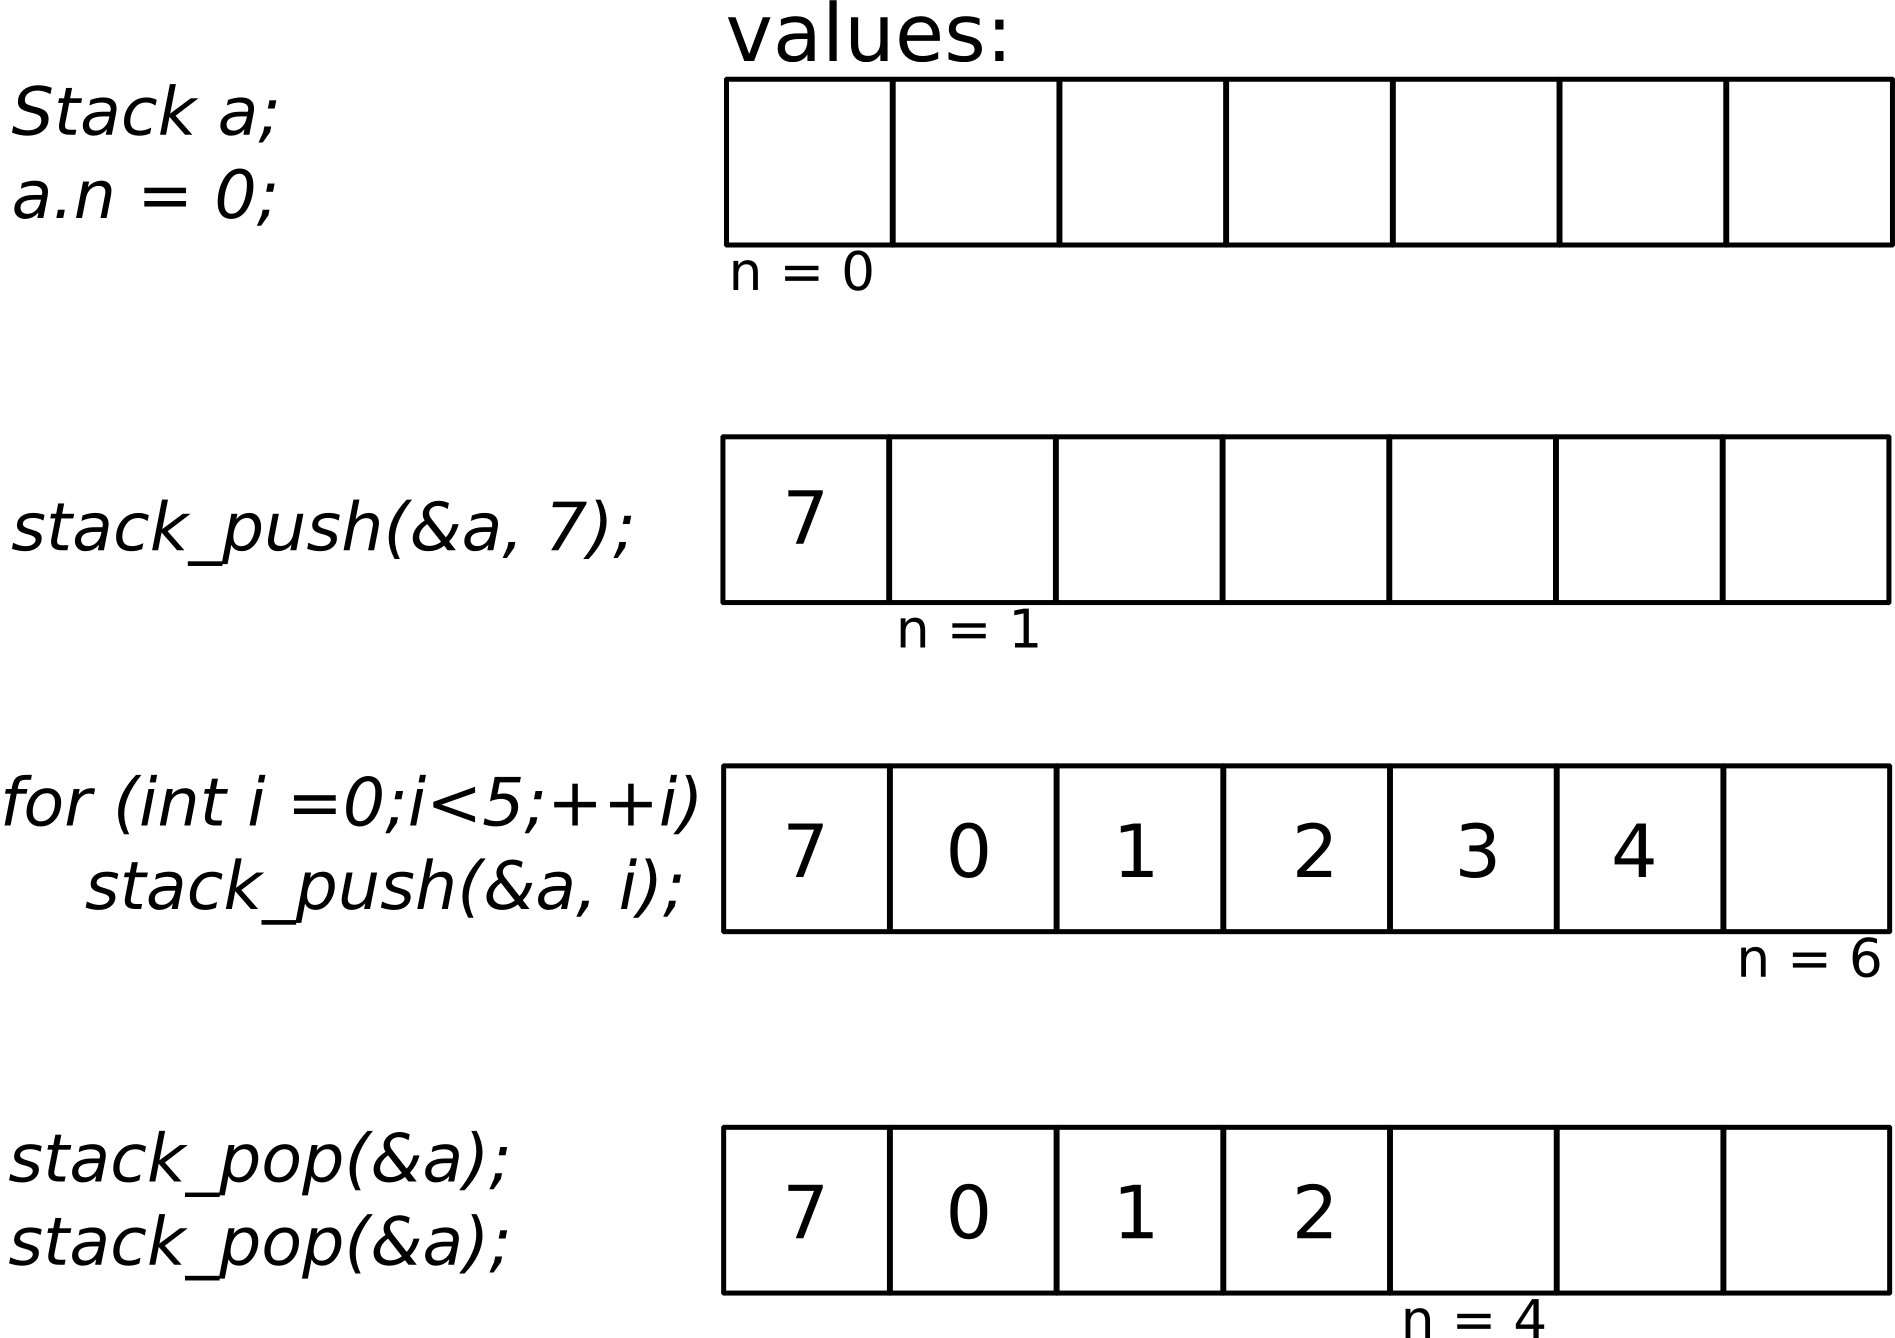
\includegraphics[width=0.95\linewidth]{../images/stack.png}
\end{center}
\end{multicols}

\subsubsection*{Задачи на связный список:}
\begin{enumerate}
\item Написать функцию \texttt{Node* list\_create()}, которая инициализирует список (просто возвращает NULL).
\item Написать функцию \texttt{void list\_add\_first(Node** p\_head, int x)}, которая добавляет элемент x в начало списка. Чтобы добавить элемент, нужно для начала выделить необходимое количество памяти под этот элемент, затем задать поля нового элемента таким образом, чтобы он указывал на начало списка. В конце нужно поменять значение указателя на начало списка. Обратите внимание, что так как нужно изменить значение указателя, то в эту функцию нужно передавать указатель на указатель.
\item Написать функцию \texttt{void list\_add\_last(Node** p\_head, int x)}, которая добавляет элемент x в конец списка. 
\item Написать функцию \texttt{int list\_remove\_first(Node** p\_head)}, которая удаляет элемент из начала списка и возвращает его значение.
\item Написать функцию \texttt{int list\_remove\_last(Node** p\_head)}, которая удаляет элемент из конца списка и возвращает его значение. 
\item Написать функцию \texttt{void list\_print(Node* head)}, которая распечатывает все элементы списка.
\item Написать функцию \texttt{int list\_size(Node* head)}, которая возвращает количество элементов списка.
\item Написать функцию \texttt{int list\_is\_empty(Node* head)}, которая возвращает 0 если список пуст и 1 если не пуст.
\item Написать функцию \texttt{int list\_destroy(Node* head)}, которая освобождает всю память, выделенную под список. Так как память выделялась под каждый элемент отдельно, то освобождать нужно также каждый элемент по отдельности.

\item Написать функцию \texttt{void list\_reverse(Node** p\_head)}, которая переворачивает связный список. Первый элемент становится последним, а последний первым. 

\item Создать структуру Stack которая будет содержать 1 элемент: указатель на Node. Написать функции \\ \texttt{void stack\_push(Stack* s, int x)}, \texttt{int stack\_pop(Stack* s)} и \texttt{void stack\_print(Stack* s)}, используя функции работы со списком.

\item Проверить работу программы с помощью valgrind. Для этого выполните в терминале \texttt{valgrind ./<имя программы>}

\item Написать функцию \texttt{int list\_concatenate(Node** p\_head1, Node** p\_head2)}, которая добавляет второй связный список в конец первого.

\item Написать функцию \texttt{int list\_is\_loop(Node* p\_head)}, которая проверяет, если в связном списке цикл.


\end{enumerate}





\end{document}